\RequirePackage[l2tabu,orthodox]{nag}

% TODO: decide if one-sided/two-sided
%\documentclass[headsepline,footsepline,footinclude=false,fontsize=11pt,paper=a4,listof=totoc,bibliography=totoc,BCOR=12mm,DIV=12]{scrbook} % two-sided
\documentclass[headsepline,footsepline,footinclude=false,oneside,fontsize=11pt,paper=a4,listof=totoc,bibliography=totoc]{scrbook} % one-sided

\usepackage{amsmath}
\usepackage[utf8]{inputenc}
\usepackage{tikz}
\usepackage[margin=2.5cm]{geometry}
\usepackage{booktabs}
\usepackage{multirow}
\usepackage{siunitx} 
\usepackage{pgfplots}
\usepackage{mathtools}
\usepackage{pgfplots}
\usepackage{tabularx, booktabs}
\usepackage{caption, subcaption}
\usepackage{adjustbox}

\pgfplotsset{compat=1.18}
\usetikzlibrary{pgfplots.groupplots}
\usetikzlibrary{positioning,calc,matrix}

% TODO: change citation style in settings
\PassOptionsToPackage{table,svgnames,dvipsnames}{xcolor}

\usepackage[utf8]{inputenc}
\usepackage[T1]{fontenc}
\usepackage[sc]{mathpazo}
\usepackage[ngerman,american]{babel}
\usepackage[autostyle]{csquotes}
\usepackage[%
  backend=biber,
  url=false,
  style=numeric,
  maxnames=4,
  minnames=3,
  maxbibnames=99,
  giveninits,
  uniquename=init]{biblatex} % TODO: adapt citation style
\usepackage{graphicx}
\usepackage{scrhack} % necessary for listings package
\usepackage{listings}
\usepackage{lstautogobble}
\usepackage{tikz}
\usepackage{pgfplots}
\usepackage{pgfplotstable}
\usepackage{booktabs}
\usepackage[final]{microtype}
\usepackage{caption}
\usepackage[hidelinks]{hyperref} % hidelinks removes colored boxes around references and links

\bibliography{bibliography}

\setkomafont{disposition}{\normalfont\bfseries} % use serif font for headings
\linespread{1.05} % adjust line spread for mathpazo font

% Add table of contents to PDF bookmarks
\BeforeTOCHead[toc]{{\cleardoublepage\pdfbookmark[0]{\contentsname}{toc}}}

% Define TUM corporate design colors
% Taken from http://portal.mytum.de/corporatedesign/index_print/vorlagen/index_farben
\definecolor{TUMBlue}{HTML}{0065BD}
\definecolor{TUMSecondaryBlue}{HTML}{005293}
\definecolor{TUMSecondaryBlue2}{HTML}{003359}
\definecolor{TUMBlack}{HTML}{000000}
\definecolor{TUMWhite}{HTML}{FFFFFF}
\definecolor{TUMDarkGray}{HTML}{333333}
\definecolor{TUMGray}{HTML}{808080}
\definecolor{TUMLightGray}{HTML}{CCCCC6}
\definecolor{TUMAccentGray}{HTML}{DAD7CB}
\definecolor{TUMAccentOrange}{HTML}{E37222}
\definecolor{TUMAccentGreen}{HTML}{A2AD00}
\definecolor{TUMAccentLightBlue}{HTML}{98C6EA}
\definecolor{TUMAccentBlue}{HTML}{64A0C8}

% Settings for pgfplots
\pgfplotsset{compat=newest}
\pgfplotsset{
  % For available color names, see http://www.latextemplates.com/svgnames-colors
  cycle list={TUMBlue\\TUMAccentOrange\\TUMAccentGreen\\TUMSecondaryBlue2\\TUMDarkGray\\},
}

% Settings for lstlistings
\lstset{%
  basicstyle=\ttfamily,
  columns=fullflexible,
  autogobble,
  keywordstyle=\bfseries\color{TUMBlue},
  stringstyle=\color{TUMAccentGreen}
}


% TODO: change thesis information
\newcommand*{\getUniversity}{Technische Universität München}
\newcommand*{\getFaculty}{School of Computation, Information and Technology}
\newcommand*{\getTitle}{From UI Images to Accessible Code: Leveraging LLMs for Automated Frontend Generation}
\newcommand*{\getTitleGer}{From UI Images to Accessible Code: Leveraging LLMs for Automated Frontend Generation}
\newcommand*{\getAuthor}{Marco Lutz}
\newcommand*{\getDoctype}{Bachelor's Thesis in Information Systems}
\newcommand*{\getSupervisor}{Sidong Feng}
\newcommand*{\getAdvisor}{Chunyang Chen}
\newcommand*{\getSubmissionDate}{11.08.2025}
\newcommand*{\getSubmissionLocation}{Munich}

\begin{document}

% Set page numbering to avoid "destination with the same identifier has been already used" warning for cover page.
% (see https://en.wikibooks.org/wiki/LaTeX/Hyperlinks#Problems_with_Links_and_Pages).
\pagenumbering{alph}
\input{pages/cover}

\frontmatter{}

\input{pages/title}
\input{pages/disclaimer}
\addcontentsline{toc}{chapter}{Acknowledgments}
\thispagestyle{empty}

\vspace*{20mm}

\begin{center}
{\usekomafont{section} Acknowledgments}
\end{center}

\vspace{10mm}

%TODO: Acknowledgments
I would like to express my appreciation to Prof. Dr. Chunyang Chen 
for providing the opportunity to conduct this thesis within the 
Chair of Software Engineering \& AI.
I am especially grateful to Sidong Feng for his direct guidance, 
constructive feedback, and continuous support, which have been 
very valuable throughout the research and writing process.

\cleardoublepage{}

\chapter{\abstractname}

%TODO: Abstract

As Multimodal Large Language Models (MLLMs) increasingly support 
UI code generation from visual inputs (e.g., UI screenshots), their impact 
in accelerating frontend development is growing. While prior work 
has explored the generation of functional and visually accurate code,
its accessibility remains less explored. This thesis 
investigated the accessibility of MLLM-generated HTML/CSS code from 
UI screenshots in an empirical study. It evaluates multiple 
state-of-the-art MLLMs with different prompting strategies 
across benchmark and real-world datasets. The study, presented 
in this thesis, investigates 
five research questions: (1) whether MLLMs can generate accessible 
code by default, (2) how model differences impact accessibility 
outcomes, (3) whether advanced prompting techniques improve 
accessibility, (4) how consistent accessibility 
violations are across different MLLMs given the same UI 
screenshot, and (5) the presence of potential data leakage
in model training. The findings show that even though MLLMs demonstrate 
high performance in code fidelity, they often fail to fulfill 
critical accessibility requirements. They also highlight common violations,
analyze prompting effects, and discuss implications for model training
and evaluation. Based on these findings, this thesis proposes future research
directions to enhance accessibility in AI-driven frontend development.
\microtypesetup{protrusion=false}
\tableofcontents{}
\microtypesetup{protrusion=true}

\mainmatter{}

% !TeX root = ../main.tex
% Add the above to each chapter to make compiling the PDF easier in some editors.

\chapter{Introduction}\label{chapter:introduction}

\section{Motivation}
High quality webpages are the backbone of our modern society. 
For billions of people the internet and thus webpages are the central access point 
for information, education, work, trade and culture. 
As of 2024, there are an estimated 1.1 billion active websites 
globally, with approximately 252,000 new sites launched each
day~\cite{web:website}.\newline
Among the many attributes that define a successful website, \emph{accessibility} stands 
out as a fundamental requirement. It ensures that individual users
with visual, hearing or cognitive
impairments, as well as users of assistive technologies, can follow the content
of a website.
International standards, such as the Web
Content Accessibility Guidelines (WCAG)~\cite{wcag21} guide developers 
to build inclusive digital experiences by adhering to the official 
principles. According to WCAG, accessible web content must be 
perceivable, operable, understandable and robust.
Yet, despite its importance, accessibility is frequently overlooked in
practice, resulting in persistent barriers for the over one billion people globally who live with some
form of disability~\cite{web:disability}.\newline
The motivation for this rethinking is not purely technical but deeply ethical and societal. It is a
legal requirement and a civil right in many jurisdictions, protected by laws such as the Americans
with Disabilities Act (ADA) in the United States~\cite{web:ADA1990} and the European Accessibility Act (EAA) in
the EU~\cite{web:EAA2019}. Neglecting to follow these regulations, could result in warnings,
reputational damage and loss of sales in the future.\newline
At the same time, Large-Language Models (LLMs) have demonstrated signifant 
improvements in code-related tasks, including code generation, completion and 
summarization. Current Tools, such as  GitHub Copilot~\cite{web:copilot}, 
Cursor~\cite{web:cursor}, Windsurf~\cite{web:windsurf},
are capable to support developers by generating functional code 
snippets from natural language descriptions. Recent developments in 
Multimodal Large Language Models (MLLMs) have further extended this capability to
\textit{Image-to-Code} tasks where based on a (UI) screenshot or design 
artifact,
MLLMs generate functional HTML/CSS code. This workflow closely aligns 
with how developers and designers intuitively approach UI
creation~\cite{chen2018ui,feng2022auto}. This image-to-code 
principle significantly simplifies the front-end development process and 
reduces the need for manual markup creation. Based on this idea,
an increasing number of research has explored techniques to improve 
UI code generation~\cite{cali2025prototype,mowar2025codea11y,wu2025ui2code}, 
leveraging MLLMs to better capture layout structures, semantics 
and component hierarchies. For instance, DCGen~\cite{wan2024dcgen}
uses a divide-and-conquer pipeline to segment UI screenshots and then 
generate code for each segment respectively. 
DeclarUI~\cite{zhou2024declarui} integrates MLLMs with advanced 
prompting strategies, particullary a self-refinement loop in which 
a multimodal model reviews and revises its draft to improve code
quality.\newline
While many MLLMs have demonstrated impressive capabilities 
in generating functional and visually accurate web UI code, 
their performance in generating accessible code remains unclear.
This question has hardly been investigated to date. 
Aljedaani et al\cite{aljedaani2024chatgpt} evaluated ChatGPT's
capabilities to generate accessible websites based on natural 
language prompts provided by developers. Similarly, Suh et 
al~\cite{suh2025accessiblecode} compared LLM-generated code
with human counterparts in terms of accessibility compliance.
However, these studies rely on natural language inputs which do
not reflect the real-world UI development workflows where visual 
UI designs (e.g. screenshots) serve as the primary input. Therefore,
this thesis tries to close this gap by investigating the capabilities 
of MLLMs to generate accessible HTML/CSS code from visual web 
UI inputs. 

\subsection{Research Questions}
The investigation is based on the following research 
questions:\newline
\textbf{RQ1: Do MLLMs generate accessible code from UI screenshots?}
This question investigates wether leading MLLMs, such as GPT-4o and 
Gemini 2.0 Flash, can generate accessible HTML/CSS code from UI 
screenshots sampled from real-world public datasets(Design2Code and 
WebCode2M). The experiment is based on a naive prompting strategy 
that requests code generation and does not explicitly instruct 
the model to prioritize accessibility. The generated code is 
then evaluated using automated accessibility auditing tools and 
manual analysis to identify potential violations of the WCAG 2.1
guidelines. This question seeks to uncover wether current MLLMs
inherently incorporate accessibility during 
code generation.\newline

\textbf{RQ2: Do different MLLMs vary in their ability to generate accessible UI code?}
To investigate how different models and their size affect the 
accessibility performance, this question compares the performance of 
a broader set of MLLMs, including both closed-source models
(e.g., GPT-4o, Gemini 2.0 Flash) and open-source
models (e.g., Qwen2.5-VL 7B). Using the same benchmark dataset and 
naive prompting approach, the numbers and types of accessibility 
violations for each model are compared. This comparison allows to
identify the differences in model behavior and analyze potential 
sources of bias or limitations in accessibility compliance. A
qualitative analysis of the generated code further explores how 
factors such as training data biases, model instructions and 
internal reasoning abilities contribute to the variance in
performance across different models.\newline

\textbf{RQ3: Does advanced prompt engineering and (post-)processing steps lead to more accessible MLLM-generated UI
code?}
This question explores wether advanced prompting strategies can guide 
MLLMs to generate more accessible code. Particularly, it investigates
the effectiveness of seven prompting strategies. Naive prompting as the
baseline, zero-shot prompting with explicit accessibility instructions,
few-shot prompting with examples of accessibility guidelines,
chain-of-thought prompting to encourage step-by-step reasoning, 
agentic prompting where multiple agents split the tasks of
detecting, classifying and solving violations. 
Lastly, two strategies use external tools to enhance their output:
ReAct prompting where the model iteratively critiques and improves 
its own output based on violations found by accessibility tools, 
color-aware prompting uses ReAct to critique its own violations, but 
further instructs the model with color contrast information and 
potential fixes. Those strategies are evaluated based on the same 
benchmark dataset across the different MLLMs and resulting violations 
are assessed. This investigation reveals the effectiveness of prompting 
as a controllable factor in improving accessibility violations, 
also highlighting potential side effects, such as cascading 
errors introduced during refinement steps. Those finding provide 
insights for developer and reseachers aiming to guide MLLMs towards 
more inclusive code generation.\newline

\textbf{RQ4: Does data leakage influence the accessibility of MLLM-generated UI code?}
To rule out potential data leakage and influence on the accessibility 
of MLLM-generated code, this question compares the models' performance across
three distinct datasets: the public benchmark dataset used in previous 
RQs, a synthetic dataset created through structural mutations and 
a fresh real-world dataset curated from open-source web projects, 
released after the knowledge cut-off of the affected MLLMs. By 
evaluating the code similarity and accessibility violations across
these datasets, this questions tries to identify wether the 
performance is driven by memorization of training data or by 
true generalization. This analysis helps to reinforce findings 
of previous RQs and ensures that observed model behaviors reflect
robust capabilities rather than overfitting to familiar data.\newline

This empirical study demonstrates both the potential and 
limitations of current MLLMs in generating accessible UI code 
from visual inputs. 
Motivated by these findings, this thesis reflects on broader implications
for the design and deployment of generative models in web development. Especially, it 
intends to rethink accessibility as a primary design objective, rather than a 
post-hoc concern. These perspectives offer possible directions for enhancing accessibility in the era of multimodal code generation.



\subsection{Our Contributions}
In summary, this thesis makes the following contributions:

\textbf{Accessibility evaluation pipeline}
The first large scale accessibility study and evaluation pipeline of LLM-based
Image-to-Code generation is proposed. This pipeline combines visual and structural 
fidelity with an automatic WCAG 2.1 conformity check.\newline

\textbf{Realistic dataset}
This study uses a realistic dataset that contains of 53 real-world webpage 
examples which have been gathered from existing datasets and slightly mutated to
minimize noise within the data. It covers a wide spectrum of layouts, content 
areas and accessibility features. This dataset combines the screenshots 
and HTML/CSS code of each webpage.\newline

\textbf{Model and prompting comparison}
This study compares multiple MLLMs and prompting strategies across diverse benchmarks and
conducts a qualitative analysis to understand their impact on the accessibility of generated code.
We release our experimental dataset, the code and the results on 
Github\footnote{\url{https://github.com/marcolutz00/Image2Code}}.\newline

\textbf{In-depth quantitative and qualitative discussion}
This study presents an in-depth discussion of our findings and proposes 
future directions for improving MLLM-driven UI-workflows.







% TODO: add more chapters here
\chapter{Related Work}\label{chapter:RelatedWork}

\section{Background}
Large Language Models (LLMs) and their performances in various domains are improving 
rapidly. Especially, in the domain of coding those models show promising results. 
It is therefore not surprising to see attempts to automate frontend code generation.

\section{Image-to-Code}
The focus of the first attempts in this area was to capture the image as precise as 
possible in order to translate it into Frontend Code. As \textit{pix2code}~\parencite{beltramelli2017pix2code} 
used a combination of CNN encoder with a LSTM decoder to translate screenshots into 
a frontend specific language. While it showed promising results for the possibility 
of end-to-end learning, it could not create standard HTML/CSS.\newline
Within the recent years, LLMs have improved a lot and new vision capabilities have been 
added to the models. Instead of further retraining models, researchers have 
explored the capabilities of different prompting structures. A prominent example is
\textit{DCGen}~\parencite{wan2024dcgen} where researchers have segmented screenshots 
into smaller, visual segments, let LLMs generate code for each segment and reassemble 
them them afterwards. This approach reduces the misplacement of components and shows
improvements in the visual similarity.\newline
Other related papers explored ways to improve prompting techniques (paper). They 
showed that advanced prompting techniques, such as few-shot, chain-of-thought and 
self-reflection can improve the performance without changing the models parameters.


\section{Web Accessibility}
asf

\section{AI-enhanced GUI testing}
adsf

\chapter{Dataset}\label{chapter:Dataset}

\section{Construction}
The main goal is to gather a diverse and high-quality dataset which represents static
real-world HTML/CSS webpages. This includes different layouts, components and contents. 
In the past, there have been different attempts to collect a dataset fullfilling
exactly those requirements.\newline
Two promising examples in this field are \textit{Design2Code} and \textit{Webcode2m}. 
Both have used existing, large datasets and applied different processing steps to 
filter bad examples and remove noise or redundancy from the code. Based on their
dataset curation, both serve as a good base for this thesis.\newline
Therefore, we decided to use both datasets and manually select 53 high-quality data 
entries. Those 53 data entries consist of 28 entries from Design2Code and 25 entries
from Webcode2m. In order to compare them on a fair basis, we only collect webpages 
that have english as their primary language.

\subsection{Content Distribution}
By using data entries of various domains and different layouts, we make sure to get 
a fair representation of the distribution of webpages in the real world. Based on 
our manual selection, we present the domain distribution in a pie chart in Figure 1.

\begin{figure*}[p]
  \centering
  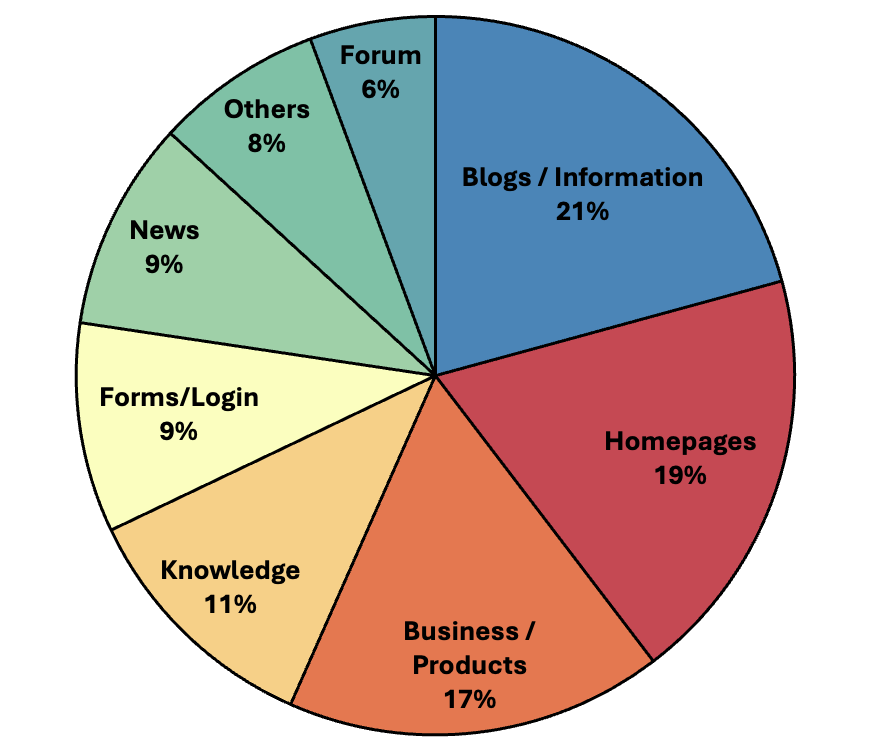
\includegraphics[width=\textwidth]{figures/dataset_distribution.png}
  \caption{Distribution of Topics in Dataset}
  \label{fig:dataset_distribution}
\end{figure*}

\section{Dataset Mutation}
Due to the fact that Design2Code and Webcode2m use different strategies to purify
their data, it is necessary to align both datasets in order to get a fair comparison.
This includes removing all external dependencies such as multimedia files (e.g. images
, audio, videos, {\ldots}) from the datasets. Furhtermore, this means adding 
placeholders like src=\"placeholder.jpg\" for images or href=\"\#\" for <a> Tags.
Lastly, we remove all of the non-visible content (advertisement-related, hidden) 
of the webpages, because it is not necessary in an Image-to-Code environment and 
could only add negatively to the accessibility score.


\section{Data Leakage}
In a last step we try to rule out the risk of data leakage. Both datasets have been
uploaded to Huggingface a few months before the official knowledge-cutoff of some of the LLMs, which
we use, and theoretically, they were publicly available at that time. 
While Design2Code has uploaded its data 3 months before the knowledge-cutoff, in the 
case of Webcode2m, it was only 2 months. To tackle this issue, we create a 
new, leakage-proof dataset of 20 entries which we input to the LLMs and compare their 
performance. If the performance in terms of our Benchmarks is comparable to our the one 
of our existing dataset, we assume that no data leakage has occurred.\newline
This test dataset has 20 data entries and has been collected the following way:

\begin{itemize}
  \item \textbf{Mutation of existing Data Entries:} We use 10 randomly-selected data entries of our existing 
  dataset. 
  \item \textbf{Collection of new Data Entries:} The other 10 data entries have been collected from 
  two Github repositories which contain frontend webpages. Those webpages have been crawled 
  and added to the dataset.
\end{itemize}

\subsection{Mutation of existing Data Entries}
The mutation of the data entries tries to change the existing ones without losing the 
reference to the real-world. The goal is to change the data entries in such a way, that
the LLMs cannot memorize the data entries, without adding artificial noise or new 
accessibility violations. Therefore, we apply the following mutations to the data entries:

\begin{itemize}
  \item \textbf{Text:} The entire text has been rewritten by a LLM. While the meaning
    and the length (max ±20 \%) remains roughly the same, the wording changes
    completely, in order to avoid memorization based on text snippets.
  \item \textbf{Text Font:} To change the visual appearance of the data entries, we 
    define a set of 5 commonly used fonts in webpages. Based on a random sample, we 
    change the text font for each data entry.
  \item \textbf{Colors:} The \textit{HUE} color code of each element is slightly
    changed based on a random shift (±20 degrees). Apart from that, the saturation
    and lightness of the color is changed by a maximum of ±20 \%.
\end{itemize}

Since those changes remain quite superficial and might not be enough to rule out 
data leakage, we further alter those data entries. We randomly change the structure 
of the data entries manually. Components, such as tables, images and text are 
interchanged within one html/css file in order to alter the webpage's layout.
Apart from that, we implement cross-web exchanges, similar to former research (paper).
We randomly select an order and exchange header and footer within different files. 
This ensures a completely new layout, while making sure that the new data entries 
remain realistic and similar to their real-world parents.

\subsection{Collection of new Data}
In a second step we collect webpages of two Github repositories which have been 
created in 2025. The first repository (source) is an educational project 
with many different webpage styles and layouts. The second repository (source)
offers a wide range of e-commerce related webpages. \newline
We crawl their html/css, pay attention on diverse content and randomly select
10 examples of this pool.


\subsection{Results}
The final results can be seen in the appendix. However, they show no difference 
in terms of the benchmarks between the existing dataset and this new leakage-free 
dataset. Since we do not have any evidence for data leakage, we assume that the 
LLMs have not seen the existing data and therefore continue with the tests.



\chapter{Benchmarks}\label{chapter:Benchmarks}

\section{Visual and Structural Similarity}
The main instruction for LLMs for this experiment remains an Image-to-Code task, where 
we input a webpage screenshot and expect a working HTML/CSS as output.
Therefore, it 
is necessary to evaluate the generated HTML/CSS code based on visual and structural
similarity. \newline
One fine-grained approach has been introduced by \textit{Design2Code}~\parencite{si2024design2code}.
It compares the input against the output based on component-level metrics rather than in its entirety.
The matching algorithm combines the 
HTML elements in the ground truth with those in the generated code. Based on this 
matching, the following metrics are calculated and combined with equal 
weights in a final score:
\begin{itemize}
  \item \textbf{Text-similarity:} Compares the text content of the HTML elements based on 
  the sequence-matching algorithm of Python's difflib library.
  \item \textbf{Position-similarity:} Evaluates the position fidelity of the HTML elements
  by comparing the bounding boxes of the elements in the ground truth and the generated code.
  \item \textbf{Color-difference:} Calculates the text color difference between two blocks 
  using the \textit{CIEDE2000} color difference formula.
  \item \textbf{Clip score:} Uses the \textit{CLIP} model to compare the visual similarity.
  \item \textbf{Area sum score:} Calculates the area of the bounding boxes and compares its
  size.
\end{itemize}
The combination of those scores allows to get a balanced view of the visual and 
structural similarity of the input and output.


\section{Accessibility Metrics}
Apart from the amount of accessibility violations, we measure and compare the 
accessibility improvements in terms of 
quantity and severity with two metrics:
\begin{itemize}
  \item The \textit{Inaccessibility Rate} (IR) has been used in previous, comparable
research~\parencite{alshayban2020accessibility}. It measures the 
percentage of DOM nodes with violations compared to the total amount of DOM nodes.
Therefore, it divides the amount of nodes with accessibility 
violations by the amount of nodes which are susceptible for violations.\newline
\begin{equation}
    \mathrm{IR} = \frac{N_{\mathrm{violations}}}{N_{\mathrm{total}}}
\end{equation}
\item To capture the severity of accessibility violations according to the WCAG impact levels,
we introduce the \textit{Impact-Weighted Inaccessibility Rate} (IWIR). It 
uses the pre-defined impacts of accessibility violations found 
(minor, moderate, serious, critical)
and assigns them to a value (1, 3, 6, 10). This scoring reflects the non-linear 
increase in impact for people with disablities, if a violation with a higher 
impact takes place within the code. Finally, we normalise the sum of all 
impact values by the worst-case scenario.\newline
\begin{equation}
  \mathrm{IWIR} = 
    \frac{\displaystyle\sum_{i=1}^{k} v_i \, w_i}
         {\displaystyle\sum_{i=1}^{k} v_i \, w_{\mathrm{max}}}
  \label{eq:iwir}
\end{equation}
\begin{table}[ht]
\centering

\caption{Severity weights used in IWIR.}
  \label{tab:weights}
  \begin{tabular}{lcc}
  \toprule
  Impact level & WCAG level & Weight $w_i$ \\
  \midrule
  Minor    & AAA          & 1  \\
  Moderate & AA or AAA    & 3  \\
  Serious  & A or AA      & 6  \\
  Critical & A          & 10 \\
  \bottomrule
  \end{tabular}
\end{table}

\end{itemize}

The combination of both metrics allows us to understand wether LLMs can not only decrease
the amount of accessibility violations, but also its severity.

\subsection{Accessibility Tools}
The accessibility compliance has become a central issue for 
developers. Nowadays, there exist many accessibility tools which are 
specialized in detecting accessibility violations. 
According to former studies, automated testing can detect up to $\sim$60\% 
of accessibility issues~\parencite{deque2023accessibility}. This makes them 
valuable for developers, however they can not replace manual testing completely.
However a combination of various tools can help to minimize the 
oversight of accessibility violations during the tests.
Therefore, we decided to use combine 3
light-weight but complementary tools for our experiment.
They work in similar ways, however they
differentiate in their approaches.
\begin{itemize}
  \item \textbf{Axe-Core (4.10.3):} The Axe-Core engine uses a \textit{zero 
  false-positives} approach. This means that the engine highlights only 
  those violations which are certain to be violations. This is a
  conservative approach which can possibly lead to \textit{false-negatives} in some cases.
  \item \textbf{Google Lighthouse Accessibility (12.4.0):} Even if Google Lighthouse Accessibility 
  works with the same axe-core engine, it found additional, complementary violations during tests.
  \item \textbf{Pa11y (8.0.0):} During tests on our dataset, we found out that pa11y has 
  strengths in detecting violations, especially in areas where the other tools
  seem to fail. Therefore, we decide to use it as our third complementary tool.
\end{itemize}

While this combination of different tools might not clear false-negatives, it can
help to minimize and reduce their occurrence.

\subsubsection{Cross-Tool Mapping}
Generally WCAG standards are based on a predefined multi-level structure. The 
\textit{principle} (perceivable, operable, understandable, robust) builds the first level 
and defines the main categories of accessibility. The second level - the 
\textit{guidelines} are based on the principles. The third level are the \textit{success
criteria} which are based on the guidelines. The success criteria are the
actual accessibility standards which can be checked. The last level - \textit{the 
techniques} are used to check the success criteria. They are more fine-grained
than success criteria and split into multiple different checks.\newline
While the operating principles of axe-core, lighthouse and pa11y are similar, their 
output varies since they operate on different reporting levels. While 
axe-core and lighthouse operate on the success criterion level, pa11y operates 
on the level of techniques. In order to aggregate the three tools 
and de-duplicate the violations found, we create a JSON mapping covering the $\sim$90 most
common WCAG techniques and $\sim$55 success criteria. 
With the help of this mapping, the output of all three tools can be combined in an 
automatic pipeline.


\chapter{Experiment}\label{chapter:Experiment}

\section{Section}

\subsection{Subsection}
\chapter{Evaluation}\label{chapter:Evaluation}


\section{Accessibility}
In order to provide a comprehensive analysis of the accessibility violations, 
we divide the analysis into 3 categories. Those categories differentiate in 
terms of quantitive and qualitive analysis as well as in its depth.

\subsection{Quantitive Analysis}
Figure x shows the quantitive analysis of the amount and type of Accessibility 
Violations found during the 3 experiment runs for each tuple of parameters.
Based on this figure, we can observe several interesting findings.\newline
Firstly, the amount and types of Accessibility Violations show a similar 
patterns across the different models. While overall \textit{gpt-4o} produced
slightly less violations, its numbers and distribution show a similar 
structure. 
Without the refinement techniques, we also see a very skewed error profile. 
Color contrast violations, as well as HTML landmark and region 
issues are the predominantly cause for at least 75\% of all violations in both
gemini's flash-2.5 and in gpt-4o model and with diverse prompting techniques.\newline
While gemini seems to have more color contrast violations, 
landmark and region rules cause more problems for the gpt-4o model. Those 
findings are confirmed across different parameters.\newline
The subsequent types of violations are in the fields of missing labels,
links without distinguishable color, issues with the HTML header and 
the size of frontend components. The results show a noticeable trend that 
only a small subset of possible WCAG violations cause non-negligible amounts 
of violations in an Image-to-Code environment. Especially in the case of 
gpt-4o, there are only 6 types of violations which cause more than 10
violations combined across all prompting techniques in our dataset.\newline
Similar to related papers in this field (paper xxx), our results also show 
that different prompting techniques only have small impact on the findings.
Even if the naive prompting approach does not instruct the LLMs to generate
code with compliance to the WCAG standards, it still only shows slightly 
increased amounts of violations than more advanced prompting techniques such as 
zero-shot or reasoning.\newline
Figure xyy shows the violations found in the ground truth HTML/CSS of our 
dataset. The human-written HTML/CSS of our dataset counts 1339 accessibility 
violations, leading to $\sim$25.26 violations per file across the whole dataset.
On the other hand, even gemini with the naive prompting technique,
the worst performing set of parameter, had a maximum of 917 accessibility 
violations, leading to $\sim$17.3 violations per file across the whole dataset.
This shows that LLMs write by default more accessible code than humans by 
incorporating the most important rules. However, as described above they 
struggle with more complex rules such as color contrast or landmarks
that require further information or thinking.

IR noch mit aufnehmen.
IW-IR noch mit aufnehmen.
Verteilung der Issues bei Human und LLms mit aufnehmen.
Bar Charts noch mit aufnehmen ohne iterative


\subsection{Qualitive Analysis}
In a first step, we analyze how consistent violations are within different 
within different experiment runs and dataset entries. Figure xy shows the 
consistency of the type and the amount of a violation by using the 
\textit{cosine-similarity}. Therefore, we analyze the type of violation
and its amount per file in vector-like structure. 
The cosine-similarity is then calculated between the vectors of the 
different experiment runs and dataset entries. This allows us to 
analyze how similar the violations are and to understand how consistent
the LLMs are in generating accessible code.

\newcommand{\vect}[1]{\begin{pmatrix}#1\end{pmatrix}}
\newcommand{\issues}{k}                   % Anzahl der Issue-Klassen
\newcommand{\vx}{\mathbf x}
\newcommand{\vy}{\mathbf y}

\begin{enumerate}
  \item \textbf{Amount of Issues}  
        For each test run and file we are counting the number of violations per class
        \[
          \left(
            \begin{array}{@{}l r@{}}
              \text{Issue}_{1}: & x_{1}\\
              \text{Issue}_{2}: & x_{2}\\
              \vdots           & \vdots\\
              \text{Issue}_{\issues}: & x_{\issues}
            \end{array}
          \right)
          \xmapsto{\text{to vector}}
          \vx \;:=\;
          \vect{x_{1}\\x_{2}\\\vdots\\x_{\issues}} \in \mathbb R^{\issues}.
        \]

  \item \textbf{Calculation of Cosine Similarity}  
        Given two experiment runs with $\vx,\vy\in\mathbb R^{\issues}$, we define
        \[
          \operatorname{cos\_sim}(\vx,\vy)=
          \frac{\vx^{\mathsf T}\vy}{\lVert\vx\rVert\,\lVert\vy\rVert}
          \quad\in[0,1].
        \]
\end{enumerate}

This cosine similarity is then plotted into a heatmap comparing the different 
experiment runs and files. The results can be seen in figure ab below. It 
is noticeable that most of the tiles show a bright color, referring to a 
high cosine similarity. The tiles with a darker color are mainly caused 
by 2 reasons. The first reason are files with only little violations 
that cause smaller cosine similarities due to the non-consistent 
distribution of violations. The second reason are randomly-generated 
files which have been mutated in such a way that they chose colors that 
comply with the Color Contrast Rules. Since overall the color constrast 
issues are one of the most common issues, this leads to a lower cosine 
similarity.\newline
Those findings are consistent different models and 
prompting techniques. This demonstrates that the accessibility issues are 
consistent across multiple runs and not caused by halluzination of the 
LLMs but are based on their training data and the underlying parameters.\newline
In a last step, the question arises why we see different results and 
violation distributions across the different models. Even though current 
LLMs are a \textit{black-box} regarding their training data and its impact, 
we can infer some possible bias based on recent accessibility studies. As 
the \textit{WebAIM 2025 Million} report~\parencite{webaim2025million} shows, 
79\% of all webpages contain low-contrast text. Similar results can be seen 
for WCAG landmark and region violations. 80,5\% of webpages contained at 
least one region, but only for 42,6\% a <main> element was present in the 
code. Other possible web-crawl training data sources like \textit{StackOverflow} 
and other forums could further bias the LLMs since they often start with 
the first <div> and omit the full page structure. This training data bias
could explain the observed differences in the amount and type of accessibility 
violations. Lastly, many of the observerd violations, such as color contrast
can be classified as more sophisticated, requiring a LLM to focus on the 
relative luminance and color contrast ratio. On the other hand, correct 
landmarks and regions require invisible semantics, apart from the raw pixel 
input of images. This semantic gap of information also requires deeper 
reasoning by the models. In conclusion, the observed violations follow 
a human bias which come from the vast training data that does not adhere 
fully to accessibility best practices.


\section{Image-to-Code Similarity}
Since Image-to-Code main task is to copy the input image as precise as possible,
we have analysed the performance across the different parameter sets to see how 
exact their results remain. The results in table as in the appendix 
indicate that the final scores decrease slightly when further accessibility 
instructions are mentioned to the LLMs. While the text and position similarity 
remains constant, the size and especially the text color similarity scores 
decrease. This is caused due to accessibility compliance that can cause the
LLMs to choose different colors and even component sizes to align with the 
WCAG issues. However, the changes in terms of the final score are very small 
and almost negligible.\newline
Overall, similar to former research gpt-4o demonstrates the best performance 
in this field by outperforming gemini flash-2.0 by a few percent.







% --------------------------------------------------------------------
% 1) FULL-WIDTH BAR CHART (Figure*)
% --------------------------------------------------------------------
\begin{figure*}[!ht]           % * = span both columns in two-column layout
\centering
\resizebox{\linewidth}{!}{     % guarantees “full page width”
\begin{tikzpicture}
\begin{axis}[
  ybar,
  bar width=3pt,
  ymin=0,   ymax=420,
  symbolic x coords={CC,LR,LB,LC,HD,SZ,TH,LG,LA,AT},
  xtick=data,
  xticklabel style={rotate=45, anchor=east},
  ylabel={Average nodes failed},
  enlarge x limits=0.15,
  legend style={
     font=\footnotesize,
     at={(0.5,0.98)}, anchor=north, legend columns=3},
  every node near coord/.append style={font=\scriptsize}
]
% ----------- DATA SERIES (EXAMPLE VALUES) -----------------
\addplot+[draw=none, fill=blue!70] coordinates {
  (CC,350) (LR,275) (LB,130) (LC,100) (HD,80)
  (SZ,12)  (TH,9)   (LG,5)   (LA,4)   (AT,2)
}; \addlegendentry{gemini-naive}

\addplot+[draw=none, fill=orange!80] coordinates {
  (CC,330) (LR,260) (LB,128) (LC,95)  (HD,77)
  (SZ,11)  (TH,8)   (LG,4.7) (LA,4.3) (AT,2.1)
}; \addlegendentry{gemini-zero-shot}

\addplot+[draw=none, fill=yellow!80] coordinates {
  (CC,330) (LR,260) (LB,128) (LC,95)  (HD,77)
  (SZ,11)  (TH,8)   (LG,4.7) (LA,4.3) (AT,2.1)
}; \addlegendentry{gemini-few-shot}

\addplot+[draw=none, fill=black!80] coordinates {
  (CC,330) (LR,260) (LB,128) (LC,95)  (HD,77)
  (SZ,11)  (TH,8)   (LG,4.7) (LA,4.3) (AT,2.1)
}; \addlegendentry{gemini-reason}

\addplot+[draw=none, fill=red!80] coordinates {
  (CC,330) (LR,260) (LB,128) (LC,95)  (HD,77)
  (SZ,11)  (TH,8)   (LG,4.7) (LA,4.3) (AT,2.1)
}; \addlegendentry{gemini-iterative}

\addplot+[draw=none, fill=green!80] coordinates {
  (CC,330) (LR,260) (LB,128) (LC,95)  (HD,77)
  (SZ,11)  (TH,8)   (LG,4.7) (LA,4.3) (AT,2.1)
}; \addlegendentry{gemini-iterative-refine-1}

\addplot+[draw=none, fill=green!20] coordinates {
  (CC,330) (LR,260) (LB,128) (LC,95)  (HD,77)
  (SZ,11)  (TH,8)   (LG,4.7) (LA,4.3) (AT,2.1)
}; \addlegendentry{gemini-iterative-refine-2}

\addplot+[draw=none, fill=purple!80] coordinates {
  (CC,330) (LR,260) (LB,128) (LC,95)  (HD,77)
  (SZ,11)  (TH,8)   (LG,4.7) (LA,4.3) (AT,2.1)
}; \addlegendentry{gemini-iterative-refine-3}


\end{axis}
\end{tikzpicture}}
\caption{Mean number of WCAG violations per rule group. Abbreviations are explained in Table~\ref{tab:abbr}.}
\label{fig:wcag-fullwidth}
\end{figure*}

% --------------------------------------------------------------------
% 2) EXPLANATORY TABLE FOR THE ABBREVIATIONS
% --------------------------------------------------------------------
\begin{table}[!ht]
\centering
\caption{Mapping of two-letter abbreviations to WCAG rule groups (used in Fig.~\ref{fig:wcag-fullwidth}).}
\label{tab:abbr}
\begin{tabularx}{\linewidth}{@{} l X @{}}
\toprule
\textbf{Abbr.} & \textbf{WCAG rule group} \\
\midrule
CC & Color Contrast: Text \\ 
LR & Landmark \& Region: Missing \& Unique Landmarks \\
LB & Label: Multiple Elements; Content Missing \\
LC & Links: Distinguishable Color \\
HD & Headings: Wrong Order; Empty \& Missing Headings \\
SZ & Size: Target Size; Element Too Small \\
TH & Tables: Table Headers \\
LG & Language: Document Lang Missing / Invalid \\
LA & Links: Missing Descriptive Content of \texttt{<a>} \\
AT & Alt-Text: Images \\
\bottomrule
\end{tabularx}
\end{table}

\chapter{Conclusion}\label{chapter:Conclusion}
This thesis has first systematically evaluated the 
accessibility of HTML/CSS code generated by state-of-the-art 
multimodal large language models (MLLMs) from UI screenshots.
While the models have shown impressive capabilities in 
the generation of syntactically valid code that closely 
mirrors the original UI image, they often reveal 
persistent accessibility violations across all 
models. Through an empirical study and analysis across 
different models, prompting techniques and datasets, 
this thesis identifies the most common accessibility 
violations and highlights gaps in the models' 
understanding of accessibility best practices.\newline
Based on these findings, the thesis discusses a potential 
paradigm shift in the approach of code generation, 
where accessibility should be rethought as a 
first-class objective in AI-driven UI development. 
As MLLMs continue to evolve, the findings of this 
thesis provide valuable insights, implications and 
possible directions for the future of more inclusive 
and responsible web development tools.
\chapter{Appendix}\label{chapter:Appendix}

\section{Results Data Leakage}
\sisetup{
  table-format = 1.4,    % maximal 1 Vorkommastelle, 4 Nachkommastellen
  detect-all            % übernimmt Schriftart/Fettdruck
}

% ---------- eigene Spaltentypen ----------
\newcolumntype{d}{S}     % „d“ steht für Dezimalspalte

\begin{table}[htbp]
\centering
\caption{OpenAI GPT-4o: Data Leakage (DL) based on 3 iterations}
\small                 % optional verkleinern
\setlength{\tabcolsep}{6pt} % enger packen, falls nötig
\begin{tabular}{
  l               % Model
  l               % Prompt
  | d        % Full Page (3 Spalten)
  | d d d d d     % Interaction Part (5 Spalten)
}
\toprule
\cmidrule(lr){3-3}\cmidrule(l){4-8}
\multicolumn{2}{c|}{\textbf{}} & {\bfseries Final Score} & {Size} & {Text} & {Position} & {Text Color} & {CLIP}\\
\midrule
% ---------------- Modell 1 ----------------
\multirow{4}{*}{DL Test Dataset} 
  & Naive & \bfseries 0.8917 & 0.8812 & 0.9701 & 0.8562 & 0.8451 & 0.906\\
  & Zero-Shot    & \bfseries 0.8889 & 0.866 & 0.9737 & 0.8543 & 0.8407 & 0.9098\\
  & Few-Shot   & \bfseries 0 & 0 & 0 & 0 & 0 & 0\\
  & Reasoning & \bfseries 0.8924 & 0.8819 & 0.9755 & 0.8498 & 0.8449 & 0.91\\
  & Iterative & \bfseries 0.8908 & 0.8819 & 0.9748 & 0.8475 & 0.8391 & 0.9109\\
  & Iterative Refine 1 & \bfseries 0.8878 & 0.8729 & 0.974 & 0.8469 & 0.8372 & 0.9081\\
  & Iterative Refine 2 & \bfseries 0.8887 & 0.8642 & 0.9771 & 0.8516 & 0.8439 & 0.9069\\
  & Iterative Refine 3 & \bfseries 0.8871 & 0.8497 & 0.979 & 0.8511 & 0.8483 & 0.9076\\
\midrule
% ---------------- Modell 2 ----------------
\multirow{4}{*}{Experiment Dataset}
  & Naive & \bfseries 0.8896 & 0.868 & 0.9661 & 0.8578 & 0.8456 & 0.9107\\
  & Zero-Shot    & \bfseries 0.8779 & 0.8124 & 0.9663 & 0.8558 & 0.8467 & 0.9083\\
  & Few-Shot   & \bfseries 0 & 0 & 0 & 0 & 0 & 0\\
  & Reasoning & \bfseries 0.8791 & 0.8348 & 0.9652 & 0.8549 & 0.8358 & 0.9048\\
  & Iterative & \bfseries 0.8854 & 0.8447 & 0.9694 & 0.8577 & 0.8412 & 0.914\\
  & Iterative Refine 1 & \bfseries 0.8786 & 0.8306 & 0.9677 & 0.858 & 0.8233 & 0.9131\\
  & Iterative Refine 2 & \bfseries 0.8767 & 0.8148 & 0.968 & 0.854 & 0.8315 & 0.915\\
  & Iterative Refine 3 & \bfseries 0.8731 & 0.811 & 0.9685 & 0.855 & 0.8181 & 0.9127\\
\midrule
% ---------------- weitere Modelle hier ----------------
% (dupliziere das obige Muster)
\bottomrule
\end{tabular}
\end{table}

\begin{table}[htbp]
\centering
\caption{Gemini-2.0-flash: Data Leakage (DL) based on 3 iterations}
\small                 % optional verkleinern
\setlength{\tabcolsep}{6pt} % enger packen, falls nötig
\begin{tabular}{
  l               % Model
  l               % Prompt
  | d        % Full Page (3 Spalten)
  | d d d d d     % Interaction Part (5 Spalten)
}
\toprule
\cmidrule(lr){3-3}\cmidrule(l){4-8}
\multicolumn{2}{c|}{\textbf{}} & {\bfseries Final Score} & {Size} & {Text} & {Position} & {Text Color} & {CLIP}\\
\midrule
% ---------------- Modell 1 ----------------
\multirow{4}{*}{DL Test Dataset} 
  & Naive & \bfseries 0.8801 & 0.7992 & 0.9685 & 0.8591 & 0.8251 & 0.9079\\
  & Zero-Shot    & \bfseries 0.8798 & 0.8297 & 0.977 & 0.8645 & 0.8141 & 0.9134\\
  & Few-Shot   & \bfseries 0 & 0 & 0 & 0 & 0 & 0\\
  & Reasoning & \bfseries 0.8683 & 0.799 & 0.9741 & 0.8541 & 0.8093 & 0.905\\
  & Iterative & \bfseries 0.8823 & 0.8298 & 0.9742 & 0.8624 & 0.836 & 0.9091\\
  & Iterative Refine 1 & \bfseries 0.8783 & 0.8297 & 0.9753 & 0.8616 & 0.8136 & 0.9112\\
  & Iterative Refine 2 & \bfseries 0.8874 & 0.8617 & 0.9774 & 0.871 & 0.8182 & 0.9086\\
  & Iterative Refine 3 & \bfseries 0.8899 & 0.8682 & 0.9773 & 0.8719 & 0.8224 & 0.9099\\
\midrule
% ---------------- Modell 2 ----------------
\multirow{4}{*}{Experiment Dataset}
  & Naive & \bfseries 0.8712 & 0.7992 & 0.9686 & 0.8591 & 0.8215 & 0.9079\\
  & Zero-Shot    & \bfseries 0.8685 & 0.7875 & 0.9687 & 0.862 & 0.8166 & 0.9094\\
  & Few-Shot   & \bfseries 0 &  0 &  0 &  0 &  0 &  0\\
  & Reasoning & \bfseries 0.868 & 0.7916 & 0.963 & 0.8594 & 0.7996 & 0.9067\\
  & Iterative & \bfseries 0.8707 & 0.7891 & 0.9686 & 0.8657 & 0.8209 & 0.9093\\
  & Iterative Refine 1 & \bfseries 0.8622 & 0.7703 & 0.9654 & 0.8616 & 0.8073 & 0.9064\\
  & Iterative Refine 2 & \bfseries 0.8676 & 0.7803 & 0.9683 & 0.8724 & 0.8132 & 0.9039\\
  & Iterative Refine 3 & \bfseries 0.8609 & 0.7708 & 0.9672 & 0.8707 & 0.7939 & 0.9017\\
\midrule
% ---------------- weitere Modelle hier ----------------
% (dupliziere das obige Muster)
\bottomrule
\end{tabular}
\end{table}






\newpage






\section{Prompts}
\definecolor{myblue}{RGB}{0,55,205}

\tikzset{
  promptbox/.style={
    draw=myblue,
    dashed,
    dash pattern=on 3pt off 2pt,
    rounded corners=6pt,
    line width=.8pt,
    font=\normalsize,
    inner sep=6pt,
    align=left,
  },
}

\newlength{\hgap}\setlength{\hgap}{6mm}   % horizontaler Abstand
\newlength{\vgap}\setlength{\vgap}{6mm}   % vertikaler Abstand

% Breite einer „normalen“ Box   (3 Stück + 2 Lücken = \textwidth)
\newlength{\boxwidth}
\setlength{\boxwidth}{\dimexpr(\textwidth-2\hgap)/3\relax}

% Breite der großen Box (nimmt zwei Spalten ein)
\newlength{\bigboxwidth}
\setlength{\bigboxwidth}{\dimexpr2\boxwidth+\hgap\relax}



\begin{figure}[ht]
\centering
\begin{tikzpicture}[node distance=\hgap]  % stellt den h-Abstand
%--------------------------------------------------------------
%  REIHE 1 – zwei Boxen
%--------------------------------------------------------------
% 1 a) Direct Prompt (linke Box oben)
\node[promptbox,
      text width=\bigboxwidth,
      anchor=north west] (direct)
{%
  \centering\bfseries Naive Prompt\\[4pt]
  \textcolor{myblue}{\emph{(Instruction):}}\\
  {\footnotesize 
  You are an expert web developer who specializes in HTML/CSS.
  Your task is to replicate the provided UI screenshot of a webpage pixel-perfectly using HTML/CSS.\newline
  \par}

  \textcolor{myblue}{\emph{[Guidelines]:}}\\
  \begin{enumerate}\itemsep2pt
    {\footnotesize \item \textbf{Layout}: Structure the markup so the spatial arrangement of every element exactly matches the screenshot.\par}
    {\footnotesize \item \textbf{Styling}: Reproduce fonts, colors, spacing, sizes, borders, shadows, and any other visual details as closely as possible.\par}
    {\footnotesize \item \textbf{Content}: Include all visible text, icons, and graphic elements.\par}
    {\footnotesize \item \textbf{Image placeholders}: Blue boxes represent images. Use `<img>` and as a source the placeholder file `src="src/placeholder.jpg"`
    to reserve space. However, the appropriate height and width is very important.\par}
    {\footnotesize \item \textbf{Delivery format}: Output only the complete HTML and CSS code in one file — no additional comments or explanations.\par}
  \end{enumerate}

   {\footnotesize  
    Now convert the following image into HTML/CSS according to these requirements.
    \par}
};

% 1 b) zweite Box oben (Beispiel: Mark Prompt)
\node[promptbox,
      text width=\boxwidth,
      right=\hgap of direct.north east,
      anchor=north west] (markTop)
{%
  \centering\bfseries Accessibility Reminder\\[4pt]
  \textcolor{myblue}{\emph{(Instruction):}}\\
  {\footnotesize It is EXTREMELY important that your HTML/CSS complies with WCAG 2.2.\\[2pt]
  Refer to the full spec if in doubt:\\ \par} 
  \href{https://www.w3.org/TR/WCAG22/}{\underline{\texttt{Link to WCAG 2.2}}}\\[4pt]
  \centering {\footnotesize Avoid any violations. \par}
};

%--------------------------------------------------------------
%  Koordinate für die zweite Reihe
%--------------------------------------------------------------
\coordinate (row2) at ($(direct.south west)+(0,-\vgap)$);

%--------------------------------------------------------------
%  REIHE 2 – drei Boxen
%--------------------------------------------------------------
% 2 a) Chain-of-Thought Prompt
\node[promptbox,
      text width=\boxwidth,
      anchor=north west] (cot) at (row2)
{%
  \centering\bfseries Zero-Shot Prompt\\[4pt]
  \textcolor{myblue}{\emph{(Instruction):}} \\[2pt]
  {\underline{\texttt{Naive Prompt}}}\\+\\
  {\underline{\texttt{Accessibility Reminder}}}
};

% 2 b) Failure-aware Prompt
\node[promptbox,
      text width=\boxwidth,
      right=\hgap of cot] (fap)
{%
  \centering\bfseries Few-Shot Prompt\\[4pt]
  \textcolor{myblue}{\emph{(Instruction):}}
  Blublub%
};

% 2 c) dritte Box unten  – Platzhalter
\node[promptbox,
      text width=\boxwidth,
      right=\hgap of fap] (extra)
{%
  \centering\bfseries Chain-of-Thought Prompt (CoT)\\[4pt]
  \textcolor{myblue}{\emph{(Instruction):}} \\[2pt]
  {\underline{\texttt{Naive Prompt}}}\\+\\
  {\underline{\texttt{Accessibility Reminder}}}\\+\\
  \centering {\footnotesize Let’s think step by step.\newline\newline
  \underline{Output Format} \\
  When you reply:\\
  1. Return ONE valid JSON object and nothing else.\\
  2. It MUST have exactly these keys:\\
  • "thoughts" – your internal reasoning\\
  • "code" – a complete HTML/CSS document as described above \par}
};

\end{tikzpicture}
\caption{Overview of Prompts.}
\end{figure}







\newpage








\section{Accessibility Violations Resolved}
\pgfplotsset{compat=1.18}                    % aktuelle Syntax

% ---------------- Farben definieren ---------------------
\definecolor{usable}{RGB}{ 54, 95,230}   % kräftiges Blau
\definecolor{unusable}{RGB}{234,127,111} % rötlicher Ton

\begin{tikzpicture}
\begin{axis}[
  % --- Achsen-/Diagramm-Eigenschaften -------------------
  xbar stacked,                 % horizontale, gestapelte Balken
  xmin=0, xmax=100,             % 0–100 %
  width=13cm, height=12cm,      % Gesamtgröße
  bar width=8pt,                % Balkendicke
  enlarge y limits=0.05,        % etwas Luft oben/unten
  xlabel={Percentage (\%)},
  axis x line*=bottom,          % nur untere x-Achse
  axis y line*=left,            % nur linke y-Achse
  ytick=data,                   % ein Tick pro Kategorie
  y tick label style={font=\small},
  % --- Legende oben -------------------------------------
  legend style={
    at={(0.5,1.06)}, anchor=south, draw=none,
    legend cell align=left, font=\small
  },
  % --- Werte im Balken (nur im 1. Plot) -----------------
  nodes near coords,
  nodes near coords style={
    font=\scriptsize\bfseries, text=white, anchor=center
  },
  every node near coord/.append style={
    /pgf/number format/.cd, fixed, precision=0,  % nur ganze %
    /tikz/.cd
  },
  % --- Kategorien (y-Achse) in genau der Reihenfolge ----
  symbolic y coords={
    Claude (Mark), Claude (CoT), Claude (Direct),
    GPT-4o (Mark), GPT-4o (CoT), GPT-4o (Direct),
    Gemini (Mark), Gemini (CoT), Gemini (Direct),
    Qwen-72B (Mark), Qwen-72B (CoT), Qwen-72B (Direct),
    Qwen-7B (Mark), Qwen-7B (CoT), Qwen-7B (Direct),
    Qwen-3B (Mark), Qwen-3B (CoT), Qwen-3B (Direct)
  }
]
% ---------- 1. Plot: Usable (blau) + Prozentzahlen -------
% ---------- 1. Plot: Usable -----------------------------
\addplot+[xbar,fill=usable] coordinates {
  (77,{Claude (Mark)})   (69,{Claude (CoT)})   (66,{Claude (Direct)})
  (81,{GPT-4o (Mark)})   (74,{GPT-4o (CoT)})   (73,{GPT-4o (Direct)})
  (64,{Gemini (Mark)})   (53,{Gemini (CoT)})   (47,{Gemini (Direct)})
  (54,{Qwen-72B (Mark)}) (43,{Qwen-72B (CoT)}) (41,{Qwen-72B (Direct)})
  (32,{Qwen-7B (Mark)})  (22,{Qwen-7B (CoT)})  (30,{Qwen-7B (Direct)})
  (18,{Qwen-3B (Mark)})  (19,{Qwen-3B (CoT)})  (17,{Qwen-3B (Direct)})
};

% ---------- 2. Plot: Unusable ---------------------------
\addplot+[xbar,fill=unusable,nodes near coords={}] coordinates {
  (23,{Claude (Mark)})   (31,{Claude (CoT)})   (34,{Claude (Direct)})
  (19,{GPT-4o (Mark)})   (26,{GPT-4o (CoT)})   (27,{GPT-4o (Direct)})
  (36,{Gemini (Mark)})   (47,{Gemini (CoT)})   (53,{Gemini (Direct)})
  (46,{Qwen-72B (Mark)}) (57,{Qwen-72B (CoT)}) (59,{Qwen-72B (Direct)})
  (68,{Qwen-7B (Mark)})  (78,{Qwen-7B (CoT)})  (70,{Qwen-7B (Direct)})
  (82,{Qwen-3B (Mark)})  (81,{Qwen-3B (CoT)})  (83,{Qwen-3B (Direct)})
};

\legend{Usable, Unusable}
\end{axis}
\end{tikzpicture}


\appendix{}

\microtypesetup{protrusion=false}
\listoffigures{}
\listoftables{}
\microtypesetup{protrusion=true}
\printbibliography{}

\end{document}
